% F09_radar_CY: Radar chart for Cyprus (CY)
% Values: Fin=0.124, Ene=0.348, Tec=0.224, Def=0.748, Cri=0.424, Log=0.941
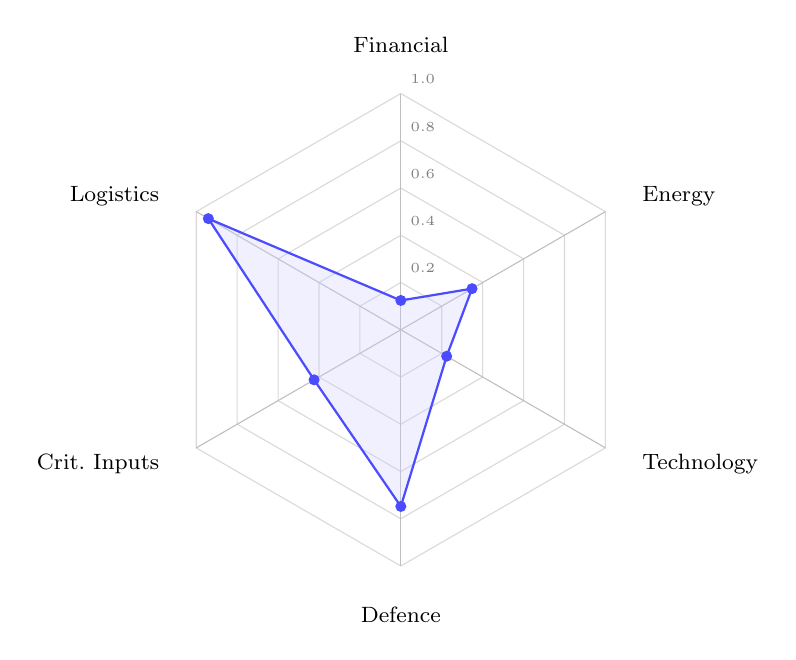
\begin{tikzpicture}[scale=1.0]
  % Grid rings
  \foreach \r in {0.2, 0.4, 0.6, 0.8, 1.0} {
    \draw[gray!30, thin]
      ( 90:\r*3cm) -- ( 30:\r*3cm) -- (330:\r*3cm) --
      (270:\r*3cm) -- (210:\r*3cm) -- (150:\r*3cm) -- cycle;
  }
  % Axis spokes
  \foreach \a in {90, 30, 330, 270, 210, 150} {
    \draw[gray!50, thin] (0,0) -- (\a:3cm);
  }
  % Axis labels
  \node[font=\footnotesize, above] at ( 90:3.4cm) {Financial};
  \node[font=\footnotesize, right] at ( 30:3.4cm) {Energy};
  \node[font=\footnotesize, right] at (330:3.4cm) {Technology};
  \node[font=\footnotesize, below] at (270:3.4cm) {Defence};
  \node[font=\footnotesize, left] at (210:3.4cm) {Crit.~Inputs};
  \node[font=\footnotesize, left] at (150:3.4cm) {Logistics};
  % Ring labels
  \foreach \r/\lab in {0.2/0.2, 0.4/0.4, 0.6/0.6, 0.8/0.8, 1.0/1.0} {
    \node[font=\tiny, gray, anchor=south west] at (90:\r*3cm) {\lab};
  }
  % Data polygon: CY
  \filldraw[blue!20, draw=blue!70, thick, fill opacity=0.3]
    ( 90:0.124*3cm) -- ( 30:0.348*3cm) -- (330:0.224*3cm) --
    (270:0.748*3cm) -- (210:0.424*3cm) -- (150:0.941*3cm) -- cycle;
  % Data points
  \fill[blue!70] ( 90:0.124*3cm) circle (2pt);
  \fill[blue!70] ( 30:0.348*3cm) circle (2pt);
  \fill[blue!70] (330:0.224*3cm) circle (2pt);
  \fill[blue!70] (270:0.748*3cm) circle (2pt);
  \fill[blue!70] (210:0.424*3cm) circle (2pt);
  \fill[blue!70] (150:0.941*3cm) circle (2pt);
\end{tikzpicture}
